\section{Mesurer un volume (3 points)}\label{ex:temperture}


\begin{questions}
	
	\begin{multicols}{2}
		
	
		\question[2] Quel volume maximal peut-on mesurer avec chacune des éprouvettes ci-contre, en $mL$, puis en $cm^3$ ?
		
		\begin{solution}
			Ces trois éprouvettes sont graduées en mL , on peut les utiliser pour mesurer un volume maximal de respectivement 50 mL, 100 mL et 250 mL. Soit 50 $cm^3$, 100 $cm^3$ et 250 $cm^3$.
		\end{solution}
		
		\question[1]	Quel est le volume de liquide contenu dans chacune des éprouvettes ?
		
		\begin{solution}
			L'éprouvette 1 contient 40 mL, la 2 90 mL et la 3 222 ml de liquide.
		\end{solution}
		
		\begin{center}
			
		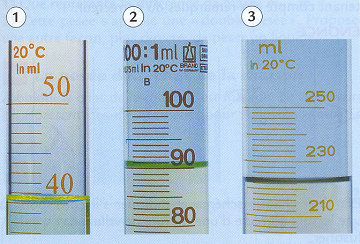
\includegraphics[scale=0.85]{img/mesure1}
		\end{center}
		
	\end{multicols}
	
\end{questions}